%----------------------------------------------------------------------------------------
%	PACKAGES AND OTHER DOCUMENT CONFIGURATIONS
%----------------------------------------------------------------------------------------

\documentclass[12pt]{article}
\usepackage[a4paper, total={6in, 8in}]{geometry}
\usepackage[english]{babel}
\usepackage[utf8x]{inputenc}
\usepackage{amsmath}
\usepackage{graphicx}
\usepackage[colorinlistoftodos]{todonotes}
\usepackage{float}
\usepackage{listings}
\usepackage{hyperref}
\usepackage{natbib}

\hypersetup{
	colorlinks   = true, %Colours links instead of ugly boxes
	urlcolor     = red, %Colour for external hyperlinks
	linkcolor    = blue, %Colour of internal links
	citecolor   = blue %Colour of citations, could be ``red''
}

\lstset{
    language=R,
    basicstyle=\ttfamily
}

\begin{document}
\bibliographystyle{apalike}

\begin{titlepage}

\newcommand{\HRule}{\rule{\linewidth}{0.5mm}} % Defines a new command for the horizontal lines, change thickness here

\center % Center everything on the page
 
%----------------------------------------------------------------------------------------
%	HEADING SECTIONS
%----------------------------------------------------------------------------------------

\LARGE Humboldt-Universit{\"a}t zu Berlin \\[0.3cm] % Name of your university/college
\LARGE School of Business and Economics  \\[0.3cm]
\LARGE Chair of Information Systems  \\[0.3cm]
\Large Applied Predictive Analytics\\[0.5cm] % Major heading such as course name
 % Minor heading such as course title

%----------------------------------------------------------------------------------------
%	TITLE SECTION
%----------------------------------------------------------------------------------------

\HRule \\[0.4cm]
{ \huge \bfseries Data Mining Cup 2015:\\[0.5cm] Basket Value Prediction}\\[0.03cm] % Title of your document
\HRule \\[1.5cm]

 
%----------------------------------------------------------------------------------------
%	AUTHOR SECTION
%----------------------------------------------------------------------------------------


\begin{table}[H]
\begin{center}
\begin{tabular}{lcr}
\emph{Submitted By:} & & \emph{Submitted To:} \\
Elisabeth Bommes & & Prof. Dr. Stefan\\
Sophie Burgard &  & Lessmann\\
Ringolf Thomschke\\ % Your name
\end{tabular}
\end{center}
\end{table}


% If you don't want a supervisor, uncomment the two lines below and remove the section above
%\Large \emph{Author:}\\
%John \textsc{Smith}\\[3cm] % Your name

%----------------------------------------------------------------------------------------
%	DATE SECTION
%----------------------------------------------------------------------------------------

{\large Summer term 2015 }\\[1cm] % Date, change the \today to a set date if you want to be precise

%----------------------------------------------------------------------------------------
%	LOGO SECTION
%----------------------------------------------------------------------------------------
\vspace{-25pt}
%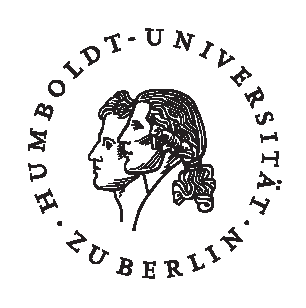
\includegraphics{husiegel_sw_op.eps}\\[1cm] % Include a department/university logo - this will require the graphicx package
 
%----------------------------------------------------------------------------------------

\vfill % Fill the rest of the page with whitespace

\end{titlepage}

\tableofcontents
\newpage

\section{Introduction}
Prudsys AG staged the 2015 Data Mining Cup (DMC) for six weeks from April 7 to May 19 2015 and we participated as part of a seminar on ``Applied Predictive Analytics''. Our two submissions ranked first and sixth place out of 188 teams from a total of 153 universities from 48 countries. 
For the 2015 Data Mining Cup, prudsys AG provided customer data from an online shop. From this data, the contestants had to predict the propensity of customers to redeem a coupon and the customers' basket value. After the release of the training and test data, the challenge was to create and submit predictions on the test data within six weeks. We divided the challenge into several different tasks which up to four team members were assigned to. In this report, we will describe the prediction of the basket value variable.\\ 

Furthermore, we extend the insight into our modeling techniques by incorporating ex post information about the values of the target variables. This knowledge is used to evaluate whether there could have been (1) problems due to the splitting of test and training sample and (2) undetected outliers and during the competition duration. We aim to answer these questions by repeatedly dividing the data set into training and hold-out samples and estimation of the respective base models and ensembles. The results are then compared by summary statistics and explorative data visualization techniques.

\section{Data}
\label{sect:data}
The initial training data set contains 6,054 observations of 33 variables. The distribution of the target variable basket value ($BV$) is right-skewed as one can conclude by comparing the estimated location parameters in Table \ref{tab:sumbv}. Note that our naming conventions of the estimated parameters are also given in Table \ref{tab:sumbv}.
\begin{table}[ht]
\centering
\begin{tabular}{cccccccc}
  \hline
  \hline
 $\hat{\mu}$ &  $\hat{\sigma}$ & Min. & Q1 & Q2 & Q3 & Max.  & Range\\ 
315.50 & 1846.07 & 46.36 & 186.30 & 212.60 & 294.10 & 135,800 & 135,828.90\\ 
   \hline
   \hline
\multicolumn{8}{l}{ \parbox{5.2in}{\vspace{1pt} \footnotesize{$\hat{\mu}$ and $\hat{\sigma}$  refer to the estimated mean and standard deviation, respectively. Q1, Q2, Q3 are the sample's first, second (median) and third Quantile. Min. and Max. are minimum and maximum and Range is defined as $Min. - Max.$}}}
\end{tabular}
\vspace{-5pt}
\caption{Summary statistics of basket value}
\label{tab:sumbv}
\end{table}
By definition of the boxplot, strong extremes may be identified as observations lying outside of the range $[Q1 - 3\hat{\sigma} , Q3 + 3\hat{\sigma}]$. We can directly isolate 237 strong extremes by this technique. 
Figure \ref{fig:histbv} shows the histogram of the basket value. One can observe that orders with a basket value of around 185 are especially frequent with more or less steadily declining frequencies of higher basket values. Also, there are two (in magnitude) smaller spikes for values smaller than 180. 
\begin{figure}[H]
\centering
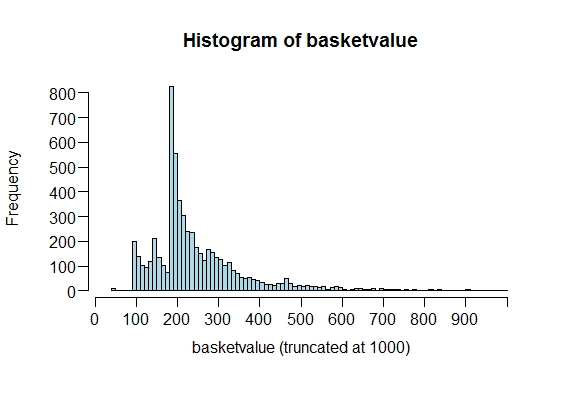
\includegraphics[width=0.83\textwidth]{histbasket.jpeg}
\vspace{-5pt}
\caption{Distribution of the basket value variable}
\label{fig:histbv}
\end{figure}
In order to stay consistent with the outlier detection and data preparation methods used for the initial competition submission, we do not try to incorporate the findings of Figure \label{ref:histbv} in the further analysis. Furthermore, we use the same procedure for outliers that is: (1) Identify outliers as $BV > 700$ and (2) if available, replace the outlier by the customer's mean basket value and otherwise by the overall mean.
We also make use of the same new variables, over 100, that have been defined during the initital competition.
The partitioning of the data set into training and test (hold-out) set is necessary to avoid overfitting during methods described in Section \ref{sect:meth}. Again, we stay in line with the original estimation and split our data set into 80\% training and 20\% test sample.\\

We also made sure that we can also build these variables for the provided prediction data set, also referred to as validation set. For example, we did not use any of the coupon usage variables to predict the basket values as they have not been available for the validation set since they are also regarded as target variables in the competition.
Prudsys published the actual values of this data sets' target variables (and hence also $BV$) after the competition ended.  

\section{Methods and Estimation}
\label{sect:meth}
We make use of the \texttt{R} package \texttt{caret} by \cite{caret} to build a library of base classifiers. The name \texttt{caret} is short for \textit{c}lassification \textit{a}nd \textit{re}gression \textit{t}raining. The package includes several different learning methods such as random forests, support vector machines and gradient boosting machines. In the further analysis, we refer to each model by using the name given in the caret package such that e.g. \texttt{qrf} stands for ``Quantile Random Forest''. 
We forego a formal discussion of these base classifiers as it would exceed the scope of this work and the descriptions can be found as well in the \texttt{caret} manual as in many textbooks. We estimate a total of 16 different base classifiers by using five-fold crossvalidation to avoid overfitting our models.
The choice of the specific models is align with \cite{Fernandez-Delgado2014} who state that various kinds of random forest models usually perform best, followed by diverse support vector machines.
The models are trained to minimize the following assessment criterion (AC) that has been given in the competition task:
\begin{equation}
AC = \sum_{i=1}^n \frac{|BV_{i} - \mbox{Pred}(BV_{i})|}{\frac{1}{n} \sum_{j=1}^n BV_{i}}
\end{equation}
with $\mbox{Pred}(\cdot)$ referring to the individual model prediction. One can observe that it is basically the Manhatten distance scaled by the factor  $\frac{1}{n} \sum_{j=1}^n BV_{i}$ and thus, models optimized using AC should be more robust against outliers than e.g. models utilizing the Euclidian distance. \\

After estimation of the base models, we use the ensemble selection techniques as described in both \cite{Caruana2006} and \cite{Caruana04}. More specifically, we implement the bagged ensemble selection method with replacement as applied by \cite{Caruana04}. The idea behing ensemble selection is to combine the predictions of all models to a single prediction which is of superior power. The data set which is used to determine the weights of each individual model in the ensemble prediction is called hillclimbing set. To avoid overfitting, the ensemble's predictive power should be assessed according a test set with observations that have not been used to either train the individual models or create the ensemble weights.\\

Up to now, there is no difference between our approach during the competition's duration and our current discussion of the results. Our main additional contribution in this seminar paper is, that we also look at the extent to which the selection of training and test set influences the performance regarding the DMC prediction data set. We repeatedly split the data set into different training and test sets to achieve this goal. Afterwards, model estimation and ensemble selection is performed for each of these sets.
This approach lets us determine how heavily the prediction performance depends on the initial choice of training and test data.  \\

Additionally, we suspect that the performance of all machine learning methods during the competition time might have been influenced by the mechanism of how to choose training and test set. During the competition, we used the texttt{caret} function \texttt{createDataPartition} to split our data set which tries to maintain the distribution of the target variable.
However, the basket value is only one of four target variables in the DMC competition as the set also includes three variables that indicate coupon usage. As for the competition submission, we intially used the first coupon variable to split the data. This way of sampling leads to an insufficiently described distribution of the basket value variable in the training sample and therefore yielding deficient prediction results. \\

We split the initial data set 98 times in different training and test set, prepare these sets according to Section \ref{sect:data} and subsequently perform model estimation and ensemble selection to investigate this matter. The previous estimation of the base models turned out to be rather tedious and time consuming, taking up to 24 hours to obtain estimates for all mentioned models. Hence, we improve the programming code by utilizing parallelization strategies in the \texttt{R} package \texttt{doParallel} by \cite{doParallel}.


\section{Results}
Firstly, we review the fit of the base models during the competition phase. We perform ensemble selection according to Section \ref{sect:meth}. The resulting weights are presented in Table \ref{tab:compens}. The models \texttt{cubist} and \texttt{parRF} obtain the largest weights and thus, represent together 80\% of the resulting ensemble prediction.

\begin{table}
	\centering
	\begin{tabular}{l|cccccc}
		\hline
		\hline
		model &\texttt{qrf} & \texttt{cubist} & \texttt{parRF} & \texttt{rf} & \texttt{RRF} & \texttt{blackboost} \\ \hline
		weight & 0.05 & 0.6 & 0.2 & 0.0985 & 0.05 & 0.0015\\
		\hline
		\hline
	\end{tabular}
	\caption{Models within the ensemble and corresponding weights}
	\label{tab:compens}
\end{table}

Table \ref{tab:compres} reports the ACs of our models, estimated by using the training data set and evaluated by either using the initial test set or the competition's validation set. The ``UserID-Model'' stands for an intuitive and probably more insightful model prepared by another group: The basket value variable is predicted by taking the mean of previous basket values for known customers while basket values of unknown customers are predicted by a simple random forest model. Clearly, this model seems to have some advantages as it both has the lowest AC for the hold-out and validation set.\\
\begin{table}
	\centering
	\begin{tabular}{l|cc}
		\hline
		\hline
		Model & AC Holdout Set & AC Validation Set \\
		& Sample (n=1210)  &  (n=669) \\\hline
		UserID-Model & 2,486 & 1,167 \\
		\texttt{cubist} & 3,355 & 1,741\\
		Ensemble & 3,390 & 1,766 \\
		\texttt{parRF} & 3,466 & 1,817 \\
		\texttt{RRF} & 3,467 & 1,816\\
		\texttt{RRFglobal} & 3,467 & 1,816\\
		\texttt{rf} & 3,468 & 1,815\\
		\texttt{qrf} & 3,472 & 1,817\\
		\texttt{ctree} & 3,475 & 1,816\\
		\texttt{cforest} & 3,485 & 1,824\\
		\texttt{gbm }& 3,469 & 1,825\\
		\texttt{blackboost} & 3,506 & 1,830\\
		\texttt{mlp} & 3,742 & 1,971\\
		\texttt{svmRadialCost} & 3,786 & 1,995\\
		\texttt{svmRadial} & 3,742 & 1,995\\
		\texttt{mlpWeightDecay} & 3,832 & 2,020\\
		\hline
		\hline
	\end{tabular}
	\caption{Evaluation of base classifiers (without obvious misclassifiers ($AC > 100,000$)}
	\label{tab:compres}
\end{table}

Other interesting findings are that the model \texttt{cubist} outperforms the ensemble selection technique while the random forest methods perform quite well and better than e.g. support vector machines as expected due to \cite{Fernandez-Delgado2014}.\\
\begin{table}[ht]
	\centering
	\begin{tabular}{cccccccc}
		\hline
		\hline
		$\hat{\mu}$ &  $\hat{\sigma}$ & Min. & Q1  & Q2 & Q3       & Max.  & Range\\ 
		1534        &      187.2      & 924.8 & 1,437 & 1,523 & 1,606 & 2,210 & 1,285.2\\ 
		\hline
		\hline
	\end{tabular}
	\vspace{-5pt}
	\caption{Summary statistics: Assessment criterion of 98 ensembles on validation sample}
	\label{tab:sumes}
\end{table}
In the next step, we investigate whether the data partitioning might have had an influence on prediction performance. Thus, we partition the data 98 times and estimate the models and perform the ensemble selection for each data set. The resulting predictions are evaluated by using the competition's validation set that was not available during the competition duration. Summary statistics of the resulting ACs can be seen in Table \ref{tab:sumes}.

Indeed, at least 75 \% of the estimated ensembles perform better than the initially estimated ensemble and base models in Table \ref{tab:compres}. More specifically, a simple check shows that this is the case for 88.78 \% of the ensembles.
However, it is also clear that only few ensembles outperform the UserID-Model (less than 25\%) and further investigation shows that this is only the case for two ensembles. \\
\begin{table}[ht]
	\centering
	\begin{tabular}{cccccccc}
		\hline
		\hline
		$\hat{\mu}$ &  $\hat{\sigma}$ & Min. & Q1  & Q2 & Q3       & Max.  & Range\\ 
		56,153        &      69,616.19     & 404 & 1,686 & 11,030 & 115,600 & 237,500 & 237,134\\ 
		\hline
		\hline
	\end{tabular}
	\vspace{-5pt}
	\caption{Summary statistics: Assessment criterion of 98 ensembles on hold-out sample}
	\label{tab:sumhold}
\end{table}

One might argue that this ex post point of view does not improve predictions during the competition phase. Thus, we select the ensemble that minimizes the AC while being evaluated by using the hold-out set. With an AC equal to $1539,612$ for the validation set it performs worse than most of the other ensembles but it is still reasonably better than the initial ensemble. However, if evaluated during the competition phase, most ensembles show a very high AC for the hold-out set. This can be clearly seen in Table \ref{tab:sumhold} and Figure \ref{tab:acensemble}. Of course, as the test set has 1,209 observations while the validation set only has 669 observations the AC evaluated on the test set should be naturally higher. However, an AC more than ten times greater seems quite excessive. One reason for these high ACs might be outliers that have not been previously recognized. \\

By taking a look on the upper part of Figure \ref{tab:acensemble}, we observe that, only two ensemble perform worse than the mean prediction on the validation set. Other observations lie rather symmetrically distributed around the AC mean. Looking at the bottom part of Figure \ref{tab:acensemble}, we realize that the ensemble with the lowest score on the hold-out sample has an average performance on the validation set. Other ensemble with slightly higher AC on their hold-out sample show better results on the validation set. Nevertheless, the very low scores on the validation set can be found in the region up to an AC value of 3,500 for the hold-out sample. Therefore, to choose an ensemble with good performance on the hold-out sample is still reasonable.
\begin{figure}[H]
	\centering
	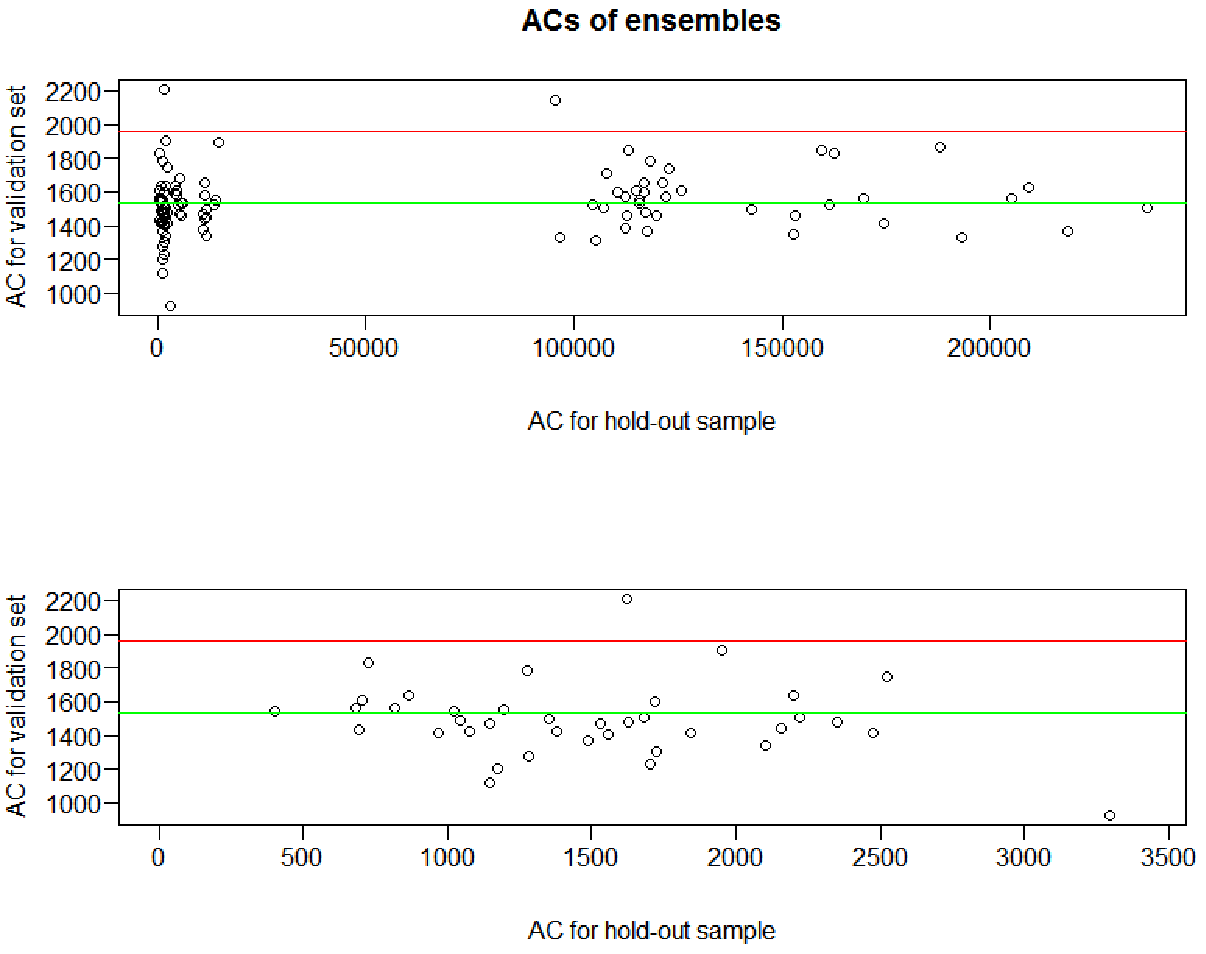
\includegraphics[width=0.83\textwidth]{ACensemble.pdf}
	\caption{Scatterplot of ACs of ensembles for hold-out sample and validation set. (Top) the entire range of ACs for hold-out sample, (bottom) truncated at 3500. Red lines indicate the AC of a mean prediction, green lines indicate the average AC on the validation set.}
	\label{tab:acensemble}
\end{figure}


\section{Conclusion}

By conducting a simulation study for the prediction of basket values with ensemble selection, we gained further insight in the importance of partitioning and detection of outliers in the context of machine learning techniques. By using differently partitioned data sets for training and testing we decreased the probability of drawing samples with different distribution than the target variable which, in general, yield bad performance measures.\\

Our first assumption was that the inferiority of machine learning models (during the competition phase) compared to the straight-forward customer mean prediction was caused by an undue partitioning of the data which did not take the target variable distribution into account. We can sustain this theory as a large percentage of estimated ensembles perform better than the initial competition ensemble. However, most of these ensembles still do not lead to better results if compared to the UserID-Model. Hence, we can conclude that a simple and smart approach which incorporates knowledge about the data might be superior in comparison to obtusely applied machine learnings algorithms. \\

We can also conclude that most ensembles perform worse on the hold-out set than on the validation set. This might be due to outliers that have not been detected in prior stages of data analysis. This emphasizes the importance of outlier handling which should be conducted with care in future competitions.

\nocite{Caruana2006}
\nocite{Niculescu-Mizil2009}

\newpage
\appendix
\section{Appendix}
R Code

\begin{itemize}
	\item Data Preparation.R
    \item Model Estimation.R
    \item Prediction Extraction.R
    \item Test Prediction.R
    \item Ensemble Selection.R
    \item Results.R
\end{itemize}

\newpage
\lstinputlisting{Data_Preparation.R}
\newpage
\lstinputlisting{Model_Estimation.R}
\newpage
\lstinputlisting{Prediction_Extraction.R}
\newpage
\lstinputlisting{Test_Prediction.R}
\newpage
\lstinputlisting{Ensemble_Selection.R}
\newpage
\lstinputlisting{Results.R}

\newpage
\bibliography{literature}


\end{document}